\documentclass{beamer}
\usetheme{metropolis}
\usepackage[utf8]{inputenc}
\usepackage[estonian]{babel}
%\usepackage[english=british]{csquotes}
\usepackage[autostyle=false]{csquotes}

\usepackage[normalem]{ulem}

\title{IDU1321. Ettevõtte äriarhitektuur}
\subtitle{Kuues loeng}
%\date{10.09.2017}
\author{Andres Kütt}
\institute{Arhitekt}


\begin{document}

\begin{frame}
\titlepage
\end{frame}



\begin{frame}[standout]
Eksami kuupäev?
\end{frame}

\begin{frame}[standout]
Ära jäänud loeng 08.12. Aga mis kell?
\end{frame}

\begin{frame}[standout]
Küsimusi kodutöö kohta?
\end{frame}

\begin{frame}[standout]
Kodutöö tagasiside
\end{frame}


\begin{frame}{Kus me oleme?}
	\begin{center}
		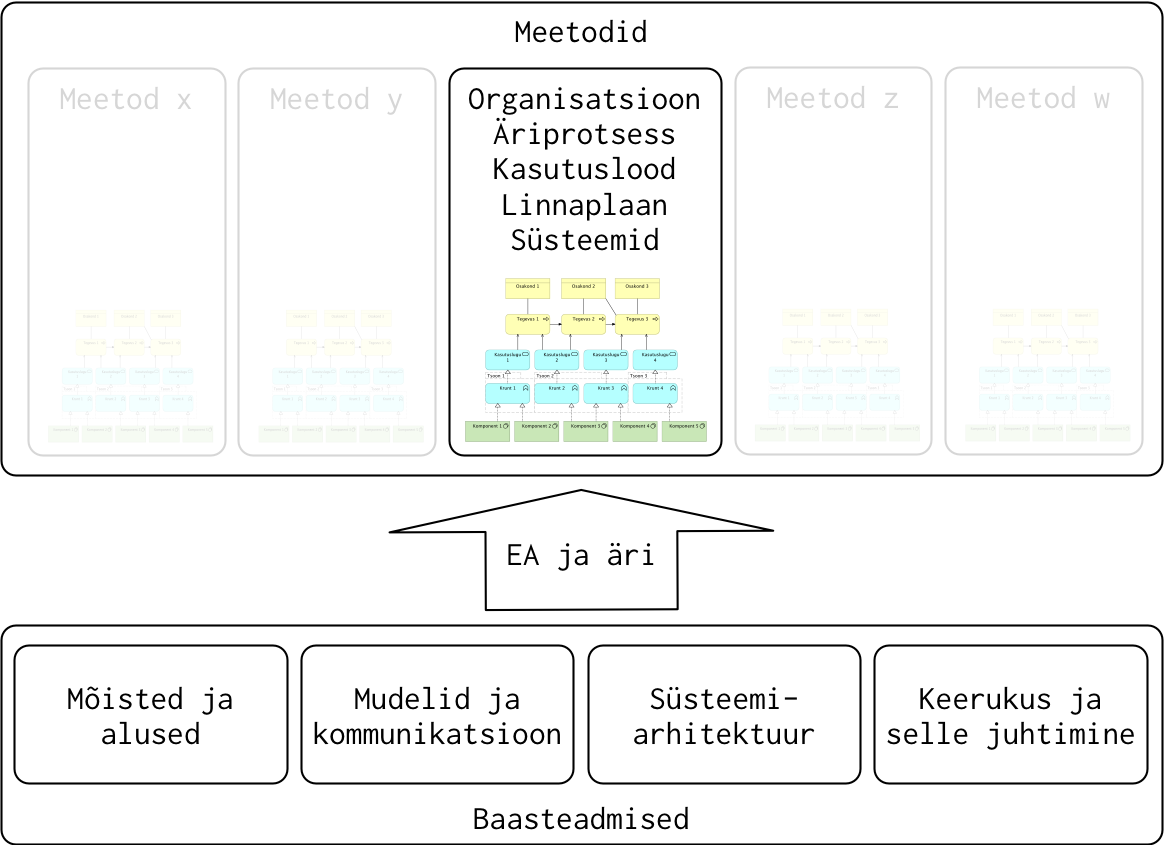
\includegraphics[width=.8\textwidth]{aine_struktuur}
	\end{center}
\end{frame}

\section{Tehniline arhitektuur}
\begin{frame}{Põgusad märkmed tehnilisest arhitektuurist}

	\begin{itemize}
		\item Põgusad, sest selle valdkonna kohta on palju sisu
		\begin{itemize}
			\item Seetõttu ka keeruline, sest kõik on spetsialistid
		\end{itemize}
		\item Selles kihis on asjad, millega töötavad programmeerijad
		\item Vahe on juhtimises: krundid on funktsionaalse ja tehnilised komponendid tehnilise juhtimise objektiks
		\item Siit allapoole ei lähe sihilikult
		\begin{itemize}
			\item Taristu arhitektuur on tänapäeval pilvest lihtsasti sisse ostetav
			\item Vajalikud kompetentsid muutuvad järsult 
		\end{itemize}
	\end{itemize}
\end{frame}

\begin{frame}[fragile]
	\begin{center}
		\LARGE{\textbf{Võtmeküsimus on \\arhitekti ja arendaja suhe}}
		\\[4cm]
		\small{Milline on teie tase \emph{selles kihis} võrreldes arendajaga? Arhitektuurikompetents koosneb teadmistest, oskustest ja kogemustest!}
	\end{center}
\end{frame}


\section{Conway seadus}
\begin{frame}{Määratlus}
	\begin{displayquote}
		Any organization that designs a system (defined broadly) will produce a design whose structure is a copy of the organization's communication structure.
	\end{displayquote}
	Melvin E. Conway
\end{frame}

\begin{frame}{Märkusi}
	\begin{itemize}
		\item Ütleb, et  organisatsioon ja tarkvara on isomorfsed
		\item Väga laialt kasutusel (Thoughtworks, agiilne kogukond jne.)
		\item Leidnud väga massilist teaduslikku kinnitust
		\item Tihti valesti interpreteeritud
		\begin{itemize}
			\item Kultuur ei ole struktuur
			\item Kommunikatsioonistruktuur on \emph{mitteametlik} struktuur, mis võib aga ei pruugi ametlikuga ühtida
		\end{itemize}
	\end{itemize}
\end{frame}

\begin{frame}{Vastasmõjust}
	\begin{itemize}
		\item Organisatsioon määrab tarkvara struktuuri kuid \textbf{vastupidist ei ole näidatud} (minu teada!)
		\begin{itemize}
			\item Kuigi isiklik empiirika kinnitab
			\item Loogika ütleb samuti nii
			\item Ma ei ole ainus, kes nii arvab
		\end{itemize}
		\item Küll aga on tõsi inerts: kommunikatsioonistruktuuri muutudes tahab muutuda ka tarkvara
	\end{itemize}
	\begin{center}
		Kas siis tarkvara struktuur võib mõjutada organisatsiooni arhitektuuri mõjutades seeläbi tarkvara struktuuri? 
	\end{center}
\end{frame}

\begin{frame}[fragile]
	\begin{center}
		\LARGE{\textbf{Põhiküsimuseks saab\\\enquote{Milline muutus on minu jaoks praegu kõige efektiivsem?}}}
		\\[4cm]
		\small{Sest kõik on kõigega seotud. Klassikaline süsteemimõtlemise järeldus: kontroll on illusioon, küsimus on meie võimes asju mõjutada ning tolle mõju tagajärgedega elada}
	\end{center}
\end{frame}

\begin{frame}{Kasutajainnovatsioon}
Kasutajad on nõus oma probleemide lahendamiseks mägesid liigutama
	\begin{itemize}
		\item \enquote{\ldots  I mean that users of products and services --- both firms and individual consumers --- are increasingly able to innovate for themselves.}\cite{hippel}
		\item \emph{Lead user} on kasutaja, kes
		\begin{itemize}
			\item \ldots toimib olulise innovatsiooni frondil ja seega kogeb esimesena asju, mida hiljem võivad kogeda paljud
			\item \ldots tajub innovatsiooni tulu/kulu bilanssi positiivsena
		\end{itemize}
		\item On näidatud, et kasutajinnovatsioon on olemuselt väärtuslik: seda peaks pigem toetama kui maha suruma
	\end{itemize}
\end{frame}


\section{Harjutus}

\begin{frame}{Lugupeetud härra Starostin}

\begin{itemize}
	\item Kontekst
	\begin{itemize}
		\item Tootmiskontsern, kõik tehased eraldi äriüksused
		\item Ühes üksuses on kohalik amatöör SCADA süsteemidega suhtlemiseks oma rakenduse teinud
		\item EU kasvuhoonegaaside turg muudab tolle andmekorje ärikriitiliseks
		\item Üksuste juhte mõõdetakse kulubaasi järgi, toimib kontsernisisene kuluarvestus
	\end{itemize}
	\item Teie kui kontserni ettevõttearhitekti ülesanne on \textbf{sõnastada probleem}
	\item Tegutsege paarides
	\begin{itemize}
		\item 18 minutit tööd probleemi formuleeringu kallal
		\item 12 minutit esitlete oma tööd kõrvalpaarile ja kuulate nende oma
	\end{itemize}
\end{itemize}
\end{frame}

\begin{frame}{Probleemiraamistik}
	\begin{itemize}
		\item Mis on probleemi liik?
		\begin{itemize}
			\item Kes/mis, kui palju, kus, millal, kuidas või miks?
		\end{itemize}
		\item Sõnasta probleem ühe lihtlausena
		\item Loetle osapooled
		\begin{itemize}
			\item Igaühe kohta märgi, kas ta on huvitatud probleemi kadumisest (+), selle säilimisest (-) või on neutraalne (N)
		\end{itemize}
		\item Loetle kasutatavad ressursid ja märgi igaühe juurde, kas tegu on \enquote{toetuspunkti} või \enquote{kangiga}
		\begin{itemize}
			\item Varad (materiaalsed ja immateriaalsed)
			\item Suhted
			\item Rgulatsioonid ja juriidika
		\end{itemize}
	\end{itemize}
\end{frame}


\begin{frame}{Harjutuse kokkuvõte}
	\begin{itemize}
		\item Kui tihti libisesite lahenduste arutellu?
		\item Mis liiki probleemiga on tegemist?
		\item Mis on peamine vara?
	\end{itemize}
\end{frame}


\begin{frame}{Kordame}
	\begin{itemize}
		\item Organisatsioon kujundab tarkvara oma näo järgi ja \emph{vist} toimib ka vastupidine
		\item Tarkvara peegeldab tegelikku ja mitte formaalset struktuuri
		\item Kontrolli saavutamise asemel keskendu efektiivsele mõjule
	\end{itemize}
\end{frame}

\begin{frame}{Järgmine kord}
\begin{itemize}
	\item Süsteemid ja nende arhitektuur
	\item Arhitektuur ja kulud
	\end{itemize}
\end{frame}

\begin{frame}{Bibliography}
	\bibliographystyle{plainnat}
	\bibliography{idu1321}
\end{frame}

\begin{frame}[standout]
Küsimusi?
\end{frame}

\end{document}
